\documentclass[fleqn]{article}
\usepackage[spanish, es-tabla]{babel}
\usepackage{amsmath}
\usepackage{amsthm}
\usepackage{graphicx}
\usepackage[utf8]{inputenc}

%%%%%%%% MARGIN
\usepackage[left=1in, right=1in, top=0.8in, bottom=0.8in]{geometry}

%%%%%%%% NO PARAGRAPH INDENT
% https://tex.stackexchange.com/questions/27802/set-noindent-for-entire-file
\setlength\parindent{0pt}

%%%%%%%% SUB-FIGURE PACKAGE
\usepackage{subcaption}

%%%%%%%% HYPERREF PACKAGE
\usepackage{hyperref}
\hypersetup{linkcolor=blue}
\hypersetup{citecolor=blue}
\hypersetup{urlcolor=blue}
\hypersetup{colorlinks=true}

%%%%%%%% MULTI-COLUMNS PACKAGE
\usepackage{multicol}

%%%%%%%% SETS DEFINITIONS
\usepackage{amssymb}
%%%% Important sets
\renewcommand{\O}{\mathbb{O}}
\newcommand{\N}{\mathbb{N}}
\newcommand{\Z}{{\mathbb{Z}}}
\newcommand{\Q}{{\mathbb{Q}}}
\newcommand{\R}{{\mathbb{R}}}

%%%% Usual operations
\newcommand{\pow}[2]{#1^{#2}}
\newcommand{\expp}[1]{e^{#1}}
\newcommand{\fst}{\mathrm{fst}}
\newcommand{\snd}{\mathrm{snd}}

%%%% Lambda Calculus
\newcommand{\dneq}{\,\, \# \,\,}
\renewcommand{\S}{\pmb{\mathrm{S}}}
\newcommand{\I}{\pmb{\mathrm{I}}}
\newcommand{\K}{\pmb{\mathrm{K}}}
\newcommand{\ch}[1]{\ulcorner #1 \urcorner}

%%%% Ordinal Lambda Calculus
\newcommand{\ordAlph}{\Sigma_{\text{Ord}}}
\newcommand{\termOrd}{\text{Term}_\text{Ord}}
\newcommand{\fl}{\mathrm{fl}}
\newcommand{\sk}{\mathrm{sk}}

%% Superscript to the left
% https://latex.org/forum/viewtopic.php?t=455
\usepackage{tensor}
\newcommand{\app}[3]{\tensor*[^{#1}]{\left(#2, #3\right)}{}}

%%%% Make optional parameter
% https://tex.stackexchange.com/questions/217757/special-behavior-if-optional-argument-is-not-passed
\usepackage{xparse}

%%%% Statistics
\NewDocumentCommand{\E}{o m}{
  \IfNoValueTF{#1}
  {\mathbb{E}\left[#2\right]}
  {\mathbb{E}^{#1}\left[ #2\right]}
}
\NewDocumentCommand{\V}{o m}{
  \IfNoValueTF{#1}
  {\mathrm{Var}\left[#2\right]}
  {\mathrm{Var}^{#1}\left[ #2\right]}
}
\RenewDocumentCommand{\P}{o o m}{
  \IfNoValueTF{#1}
  {\IfNoValueTF{#2}
    {\mathrm{P}\left(#3\right)}
    {\mathrm{P}^{#2}\left(#3\right)}}
  {\IfNoValueTF{#2}
    {\mathrm{P}_{#1}\left(#3\right)}
    {\mathrm{P}_{#1}^{#2} \left(#3\right)}}
}

%%%% Lambda Calculus
\NewDocumentCommand{\cx}{o}{
  \IfNoValueTF{#1}
  {\left[\quad\right]}
  {\left[\, #1 \,\right]}
}

%%%% Create absolute value function
% https://tex.stackexchange.com/questions/43008/absolute-value-symbols
\usepackage{mathtools}
\DeclarePairedDelimiter\abs{\lvert}{\rvert}%
\DeclarePairedDelimiter\norm{\lVert}{\rVert}%
\makeatletter
\let\oldabs\abs
\def\abs{\@ifstar{\oldabs}{\oldabs*}}
%
\let\oldnorm\norm
\def\norm{\@ifstar{\oldnorm}{\oldnorm*}}
\makeatother


%%%%%%%% LOGIC TREES
\usepackage{prftree}

%%%%%%%% SPLIT EQUATIONS
% https://tex.stackexchange.com/questions/51682/is-it-possible-to-pagebreak-aligned-equations
\allowdisplaybreaks

%%%%%%%% EXAM PACKAGE
\usepackage{mathexam}

%%%%%%%% CHANGE MARGINS ITEMIZE
\usepackage{enumitem}

\usepackage{float}
\usepackage{multirow}
\renewcommand{\u}{\mathbf{u}}
\renewcommand{\v}{\mathbf{v}}

%%%%%%%% START DOCUMENT

\ExamClass{ÁLGEBRA EN C.d.l.D}
\ExamName{EXAMEN 2}
\ExamHead{\today}

\let\ds\displaystyle

\begin{document}
 \vspace{0.3cm}
   % Information of the student
   \begin{itemize}[leftmargin=6.25cm, labelsep=0.5cm]

     \item[\textit{Nombres}] \scalebox{1.2}{Andrés Felipe Tamayo} \\
     \scalebox{1.2}{David Plazas Escudero} \\
       \scalebox{1.2}{Juan Sebastián Cárdenas Rodríguez}

   \end{itemize}
\vspace{0.3cm}

% Each of the items to solve
\begin{enumerate}
  \item Sea $X\in \mathbb{R}^{n\times p}$ una matriz de datos. Si consideramos
    la matriz de datos centrada, $\tilde{X}=PX$ donde
    $P=I_n - \frac{1_n1^T_n}{n}$ es la matriz de centrado, podemos interpretar a
    $\u$ y $\v$ como columnas de la matriz $\tilde{X}$ (las muestras asociadas a
    dos variables en particular).
    %
    Denotemos como $Y_\u$ y $Y_\v$ a las variables aleatorias asociadas a las
    columnas (vectores) $\u$ y $\v$ de la matriz de datos. Es claro que como la
    matriz $\tilde{X}$ está centrada, $\E{Y_\u}=\E{Y_\u}=0$. Recordemos que la
    covarianza entre las variables aleatorias $Y_\u$ y $Y_\v$ está dada por:
    %
    \begin{equation}
      \mathrm{Cov}[Y_\u,Y_\v] = \E{Y_\u Y_\v} - \E{Y_\u}\E{Y_\v}=\E{Y_\u Y_\v},
    \end{equation}
    %
    y usando un argumento similar se verifica que $\V{Y_\u}=\E{Y_\u^2}$ y
    $\V{Y_\v}=\E{Y_\v^2}$. Como estamos trabajando bajo una muestra finita de
    datos, se tendrían estimadores para estos valores. Asumiendo entonces que
    $\u=[u_1,\,\ldots,\,u_n]^T$ y $\v=[v_1,\,\ldots,\,v_n]^T$, si utilizamos la
    corrección insesgada de los estimadores de máxima verosimilitud, tenemos que
    %
    \[
    \E{Y_\u^2}=\dfrac{1}{n-1}\sum_{i=1}^n u_i^2,\quad \E{Y_\v^2}=\dfrac{1}{n-1}\sum_{i=1}^nv_i^2, \quad \E{Y_\u Y_\v}=\dfrac{1}{n-1}\sum_{i=1}^n u_iv_i.
    \]
    %
    Analizando cuidadosamente estas fórmulas, nos podemos dar cuenta que
    corresponden con el producto interno y norma en un espacio euclídeo, luego
    %
    \[
    \E{Y_\u^2}=\dfrac{\norm{\u}^2_2}{n-1},\quad \E{Y_\v^2}=\dfrac{\norm{\v}^2_2}{n-1}, \quad \E{Y_\u Y_\v}=\dfrac{\langle\u, \v\rangle_2}{n-1}.
    \]
    %
    Por otra parte, el coseno entre los dos vectores $\u$ and $\v$ en el espacio
    euclídeo puede ser escrito como
    %
    \[
    \cos\theta = \dfrac{\langle\u,\v\rangle_2}{\norm{\u}_2\norm{\v}_2}.
    \]
    %
    Por lo tanto,
    %
    \[
    \cos\theta = \dfrac{\langle\u,\v\rangle_2}{\norm{\u}_2\norm{\v}_2} = \dfrac{\E{Y_\u Y_\v}}{\sqrt{\E{Y_\u^2}\E{Y_\v^2}}}=\dfrac{\mathrm{Cov}[Y_\u,Y_\v]}{\sqrt{\V{Y_\u} \V{Y_\v}}}=\rho(Y_\u,Y_\v).
    \]
    %
    Luego, $\cos\theta$ puede ser interpretado estadísticamente como el
    coeficiente de correlación de Pearson entre las variables aleatorias $Y_\u$
    y $Y_\v$, de donde se puede también verificar que la correlación de pearson
    satisface $\rho(Y_\u,Y_\v)\in[-1,1]$.
    %
    Simulando una distribución normal bivariante, se obtuvieron los siguientes
    resultado:
    \begin{table}[H]
      \centering
      \begin{tabular}{lll}
        \hline
        $\cos{\theta}$ & $\rho(Y_{u}, Y_{v})$ & $|\cos{\theta} - \rho(Y_{u}, Y_{v})| $ \\ \hline
        $0.4389460$   & $0.4389477$ & $1.753822 \times 10^{-6}$   \\
        \hline
      \end{tabular}
    \end{table}
    %
    Se observa que dan resultados cercanos.

  \item La descomposición en valores singulares en imagenes permite comprimir la
    imagen, de tal forma que se puede representar la misma imagen con una matriz
    que posee menos información comparando memoria física, es decir el peso en
    el disco duro. En la Tabla \ref{tab:pesos} se pueden encontrar los pesos de
    cada imagen utilizando dos descomposiciones distintas.
    %
    \begin{table}[H]
      \centering
      \begin{tabular}{ll}
        \hline
        \textbf{Peso imagen} \\ \hline
        $\sigma_{1}$   & $14k$   \\
        $\sigma_{50}$   & $20k$    \\
        Original & $22k$ \\ \hline
      \end{tabular}
      \caption{Peso de cada imagen.}
      \label{tab:pesos}
    \end{table}
    %
    Además de que se denota una mejora suficiente en el peso de la imagen, estas
    imagenes exportadas poseen un borde blanco que incrementa el peso real. Sin
    embargo, se ilustra lo deseado. En las siguientes figuras, se observa cada
    una de las imagenes con diferentes valores singulares.
    %
    \begin{figure}[H]
      \centering
      \begin{subfigure}[b]{0.45\textwidth}
        \centering 
\includegraphics[scale=.6]{figs/exercise-2-svd-1}
        \caption{Compresión hasta $\sigma_{1}$.}
      \end{subfigure}
      %
      \begin{subfigure}[b]{0.45\textwidth}
        \centering 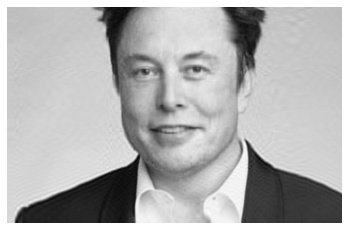
\includegraphics[scale=0.6]{figs/exercise-2-svd-50}
        \caption{Compresión hasta $\sigma_{50}$.}
      \end{subfigure}
    \end{figure}

  \item La varianza generalizada de una variable vectorial aleatoria
    p-dimensional $X$ se define como el determinante de su matriz de covarianza,
    utilizando por ejemplo la estimación de Ledoit-Wolf, OAS, MCD o algún otro
    basado en correlación robusta, como el coeficiente de Spearman o el Tau de
    Kendall.
    \begin{figure}[H]
      \centering
      \includegraphics[scale=.5]{figs/exercise-4}
      \caption{Varianza generalizada para diferentes matrices.}
    \end{figure}

  \item En analítica de datos se trabaja con una matriz de datos
    $X\in\mathbb{R}^{n\times p}$. Si retomamos la matriz de datos centrada
    $\tilde{X}$ y definimos la matriz de covarianza de $\tilde{X}$ como
    $S=\frac{\tilde{X}^T\tilde{X}}{n}$, se puede ver entonces que la
    descomposición espectral de $S$ es completamente equivalente a la
    descomposición en valores singulares de la matriz
    $\frac{\tilde{X}}{\sqrt{n}}$ mediante la transformación de raíz cuadrada: la
    descomposición en valores singulares de una matriz $A$ cualquiera es
    equivalente a hacer la descomposición espectral de la matriz $A^TA$ y los
    valores singulares serán la raíz cuadrada de los valores propios de $A^TA$.
    Luego, los valores singulares de $\frac{\tilde{X}}{\sqrt{n}}$ son la raíz
    cuadrada de los valores propios de $\frac{\tilde{X}^T\tilde{X}}{n}=S$, es
    decir, de los valores propios de la matriz de covarianza.

    Para cualquier matriz $A\in\mathbb{R}^{m\times n}$ se cumple que
    $A^TA\in\mathbb{R}^{n\times n}$ y $AA^T\in\mathbb{R}^{m\times m}$. Luego, se
    verifica que si $\lambda\neq0$ es un valor propio de $A^TA$, debe cumplir
    que
    \[
    A^TAx=\lambda x,
    \]
    para algún $x\neq0$. Premultiplicando por $A$, se tiene
    \[
    AA^T(Ax)=\lambda(Ax)
    \]
    de donde $\lambda$ también es un valor propio para $AA^T$. Los valores
    propios restantes (en caso de que $m\neq n$) deben ser 0.

  \item La norma de Frobenius de una matriz $A \in \mathbb{R}^{n \times n}$ está
    definida como $\norm{A}_{F} = \sqrt{\textbf{Tr}A^{T}A}$ dónde $\textbf{Tr}$ es
    la traza de una matriz. Probar que esta norma es invariante ante rotaciones
    de los datos es equivalente a probar que si $U$ y $V$ son ortogonales,
    entonces $\norm{UA}_{F} = \norm{AV}_{F} = \norm{A}_{F}$ y por esto, la norma de
    Frobenius no cambia por una pre ó pos transformación ortogonal.
    \begin{proof}
      Primero, notese que $\norm{UA}_{F} = \norm{A}_{F}$ porque
      \begin{align*}
        \norm{UA}_{F}^{2} &= \textbf{Tr}(UA)^{T}(UA) \\
                          &= \textbf{Tr}A^{T}U^{T}UA \\
                          &= \textbf{Tr}A^{T}A = \norm{A}_{F}^{2}
      \end{align*}
      Además, $\norm{AV}_{F} = \norm{A}_{F}$ ya que
      \begin{align*}
        \norm{AV}_{F}^{2} &= \textbf{Tr}(AV)^{T}(AV) \\
                       &= \textbf{Tr}(AV)(AV)^{T} \\
                       &= \textbf{Tr}AVV^{T}A^{T} \\
                       &= \textbf{Tr}AA^{T} \\
                       &= \textbf{Tr}A^{T}A = \norm{A}_{F}^{2}
      \end{align*}
    \end{proof}
    %
    Para mostrar esto, haremos las siguentes transformaciones ortonormales:
    %
    \begin{multicols}{2}
      \noindent
      \begin{equation*}
        \Theta_1 =
        \begin{bmatrix}
          \cos{\theta}& -\sin{\theta} \\
          \sin{\theta}& \cos{\theta}
        \end{bmatrix}, \quad \text{ with } \theta = \frac{\pi}{3}
      \end{equation*}
      %
      \columnbreak \vspace{0.5cm}
      %
      \begin{equation*}
        \Theta_2 =
        \begin{bmatrix}
          1 & 0 \\
          0 & -1
        \end{bmatrix}
      \end{equation*}
    \end{multicols}
    \vspace{-1cm}
    \begin{equation*}
      \Theta_3 =
      \begin{bmatrix}
        0 & 0 & 0 & 1\\
        0 & 0 & 1 & 0\\
        1 & 0 & 0 & 0\\
        0 & 1 & 0 & 0
      \end{bmatrix}
    \end{equation*}
    %
    En las siguientes gráficas se observa la norma de la matriz original
    comparada con la norma de la matriz desplazada. Se puede observar que estas
    normas tienen dependencia lineal y son iguales.
    \begin{figure}
      \centering
      \begin{subfigure}[b]{0.45\textwidth}
        \centering \includegraphics[scale=.45]{figs/exercise-5-sin}
        \caption{Norma utilizando $\Theta_{1}$.}
      \end{subfigure}
      %
      \begin{subfigure}[b]{0.45\textwidth}
        \centering \includegraphics[scale=.45]{figs/exercise-5-reflection}
        \caption{Norma utilizando $\Theta_{2}$.}
      \end{subfigure}

      \begin{subfigure}[b]{0.45\textwidth}
        \centering \includegraphics[scale=.45]{figs/exercise-5-perm}
        \caption{Norma utilizando $\Theta_{3}$.}
      \end{subfigure}
    \end{figure}

  \item Para encontrar los mejores métodos, se hallaron la solución del sistema
    utilizando los diferentes métodos y se halló la distancia entre $\hat{b}$ y
    el vector original. En la siguiente tabla, se observan cada una de las
    distancias para diferentes vectores.
    %
    \begin{table}[H]
      \centering
      \begin{tabular}{ll}
        \hline
        \multicolumn{2}{c}{\textbf{Distancia al vector $b$}} \\ \hline
        Solución de la inversa   & $1072087.40$   \\
        Solución de la pseudo-inversa   & $136.63$    \\
        Solución LU & $163.48$ \\
        Solución QR & $117.15$ \\ \hline
      \end{tabular}
    \end{table}
    %
    Se observa que la descomposición QR es la mejor.

  \item En la Tabla \ref{tab:coeffs} se observa los resultados de la regresión
    lineal y utilizando la pseudo-inversa.
    %
    \begin{table}[H]
      \centering
      \begin{tabular}{cc}
        \hline
        \multirow{5}{*}{Pseudo-inversa}
        &$4.994$\\
        &$3.997$\\
        &$3.666$\\
        &$3.501$ \\
        &$3.403$ \\
        \hline
        \multirow{5}{*}{Modelo de regresión}
        &$4.994$\\
        &$3.997$ \\
        &$3.666$ \\
        &$3.501$ \\
        &$3.403$ \\
        \hline
        \multirow{1}{*}{Distancia} &$1.140 \times 10^{-13}$\\
        \hline
      \end{tabular}
      \caption{Coeficientes obtenidos.}
      \label{tab:coeffs}
    \end{table}

    En primer lugar, se observa bajo la construcción de la salida $y$, que la
    fórmula está dada por
    \begin{align*}
      y &= \sum_{i=1}^5 \frac{2 + 3i}{i}X_i + \epsilon \\
        &= 5X_1 + 4X_2 + \frac{11}{3}X_3 + \frac{14}{4}X_4 + \frac{17}{5}X_5 + \epsilon \\
        &\approx 5X_1 + 4X_2 + 3.67X_3 + 3.5X_4 + 3.4X_5 + \epsilon
    \end{align*}
    %
    De esta manera, se ve que este proceso es una aproximación a los
    coeficientes de cada una de las variables. Así, esto mismo se observa que
    son los mismos valores obtenidos por mínimos cuadrados ordinarios.
\end{enumerate}
\end{document}
